\documentclass[12pt]{beamer}
\usepackage[utf8]{inputenc}
\usepackage{graphicx}

\graphicspath{ {./images/} }



\usetheme{PaloAlto}
\usecolortheme{rose}


\title{A Machine Learning-Enabled Study of Superconductivity}
\subtitle{Application of the XGBoost Algorithm}

\author[Rajeev Atla]
{Rajeev Atla}

\institute[JPS]
{
  John P. Stevens High School
}



\begin{document}




\frame{\titlepage}

\section{Introduction}

\begin{frame}
\frametitle{Outline}
\tableofcontents

\end{frame}


\subsection{XGBoost}



\begin{frame}
\frametitle[allowframebreaks]{Introduction}
\framesubtitle{XGBoost}
\begin{itemize}
  \item<1-> eXtreme Gradient Boosting
  \item<2-> Package for \textbf{Python}, C++, Java, R, Julia, and Scala
  \item<3-> Was used to process data from Large Hadron Collider (LHC) [Chen 2015]
  \begin{itemize}
    \item<4-> Won the Higgs Boson Machine Learning Challenge
  \end{itemize}
  \item<5-> Ensemble learning [\textit{Elements of Statistical Learning} Chapter 16]
  \begin{itemize}
    \item<6-> Combination of homogenous weak learners
    \item<7-> End result is a weighted sum of weak learners
    \[\theta_f = \sum \limits_{j} w_j \theta_j\]
    \item<8-> \(w_j\) are determined by backpropogation via gradient descent
  \end{itemize}
\end{itemize}
\end{frame}


\subsection{Superconductivity}
\begin{frame}
\frametitle{Introduction}
\framesubtitle{Ginzburg-Landau Theory}
\begin{itemize}
  \pause
  \item For a homogenous superconductor, the Ginzburg-Landau equation is
  \[\alpha \phi + \beta |\phi|^2 \phi = 0\]
  \pause
  \item The nontrivial solution for $T<T_c$ is
  \[ |\phi|^2 = - \frac{\alpha}{\beta} \left (T - T_c \right)\]
  \pause
  \item The characteristic length scale \(\xi \) is called the Ginzburg-Landau coherence length
  \[\xi = \sqrt{\frac{\hbar^2}{2m^{*} |\alpha| }}\]
\end{itemize}

\end{frame}



\begin{frame}
\frametitle{Introduction}
\framesubtitle{Types of Superconductors}


\begin{itemize}

  \item Two types - Type 1 and Type 2

  \pause

  \item Notation

  \pause

  \begin{itemize}
    \item \(H_c (T)\) is critical field as a function of temperature
    \pause
    \item \(T_c\) is critical temperature
  \end{itemize}

  \pause

  \begin{figure}[h]
    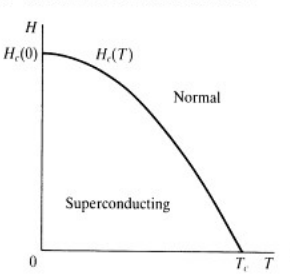
\includegraphics[scale = 0.5]{Type1.png}
    \caption{\textbf{\(H-T\) phase diagram for a Type 1 superconductor [Tinkham]}}
  \end{figure}

\end{itemize}


\end{frame}

\begin{frame}
\frametitle{Introduction}
\framesubtitle{Type 2 Superconductors}

\begin{itemize}
  \pause
  \item Ginzburg-Landau parameter \(\kappa > \frac{1}{\sqrt{2}}\)
  \pause
  \begin{itemize}
    \item Definition: \(\kappa = \frac{\lambda}{\xi} = \frac{e \hbar}{m_e c} \sqrt{\frac{\beta}{2 \pi}} \)
    \item Surface energy is negative
  \end{itemize}
  \pause
  \item \(H_{c2} = H_{c1} \kappa \sqrt{2}\)
  \pause
  \item In type 1, \(H_{c2} = H_{c1}\)
  \pause
\end{itemize}

\begin{figure}[h]
  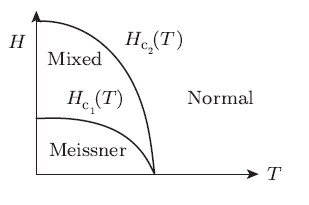
\includegraphics[scale = 0.5]{Type2.png}
  \caption{\textbf{\(H-T\) phase diagram for a Type 2 superconductor [Girvin and Yang 2019]}}
\end{figure}



\end{frame}

\begin{frame}
\frametitle{Introduction}
\framesubtitle{Type 2 Superconductors: Abrikosov Lattice Vortices}

\begin{itemize}
  \item For $H_{c1}<H<H_{c2}$ in a Type 2 Superconductor, Abrikosov vortices appear in the material
  \pause
  \item These are flux vortices that are quantized, with
  \[\Phi = \frac{nhc}{2e}, \,  \, \, \, n \in \mathbb{Z}\]
\end{itemize}
\pause
\begin{figure}[h]
  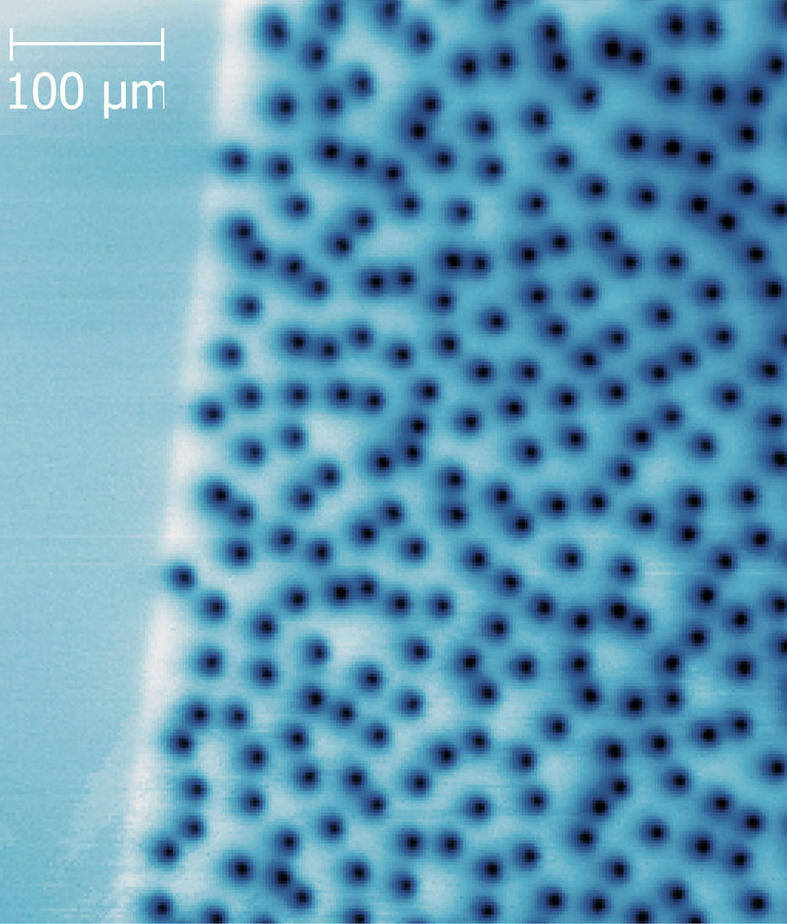
\includegraphics[scale = 0.08]{YBCO_vortices.jpg}
  \caption{\textbf{Abrikosov vortices in YBCO - created by Wells et al. 2015 using scanning SQUID microscopy}}
\end{figure}
\end{frame}

\section{Data}
\begin{frame}
\frametitle{Data}

\begin{itemize}
  \item Taken from UCI (University of California, Irvine) Machine Learning Repository
  \pause
  \item 21,263 examples with 81 features
  \pause
  \item Model was only trained with 11 features to prevent overfitting
  \pause
\end{itemize}

\begin{figure}[h]
  
\includegraphics[scale = 0.5]{UCIRepo.png}
  \caption{\textbf{UCI Machine Learning Repository}}
\end{figure}

\end{frame}



\section{Methods}



\begin{frame}
\frametitle{Methods}

\pause
\begin{itemize}
  \item XGBoost library
  \begin{itemize}
    \pause
    \item XGBClassifier class
  \end{itemize}
\end{itemize}

\end{frame}



\section{Discussion}

\begin{frame}
\frametitle{Discussion}
\pause
\begin{itemize}
  \item Confusion matrix made using matplotlib library
\end{itemize}
\pause
\begin{figure}[h]
  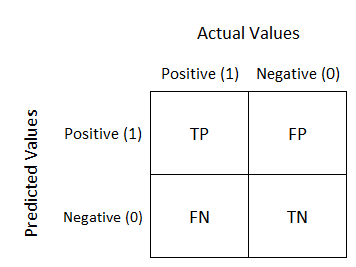
\includegraphics[scale = 0.5]{confusionmatrix.png}
  \caption{\textbf{Example Confusion Matrix}}
\end{figure}

\end{frame}

\section{Conclusion}

\begin{frame}
\frametitle{Conclusion}
\pause
\begin{itemize}
  \item Python training files, these slides, the dataset, etc. can be found at \url{https://github.com/RajeevAtla/Graphene-Research/}
  \pause
  \item Easiest way to access is using git
\end{itemize}



\end{frame}

\section{References}
\begin{frame}
\frametitle{References}
\end{frame}


\section{Acknowledgements}


\begin{frame}
\frametitle{Acknowledgements}
I would like to thank Leo Lo and Dr. Serena McCalla for their mentorship through the iResearch Institute.

\begin{center}

\includegraphics[scale = 0.58]{iresearch.png}
\end{center}

I would also like to acknowledge my parents for their constant support.
\end{frame}









\end{document}
